\chapter{The Chocolate Cake}
\label{ch:chocolatecake}
\index{dessert}
\index{cake}
\index{chocolate}
\textit{A Very Chocolatey Cake with Syrup and Maraschino Cherries}

Family member: Grandma Eleni


\marginnote[20pt]{\\
    \textbf{Makes 1 cake} \\
    Prep time: ? minutes \\
    Cook time: ? minutes \\
    \vspace*{\baselineskip}

    \textbf{Ingredients for cake} \\
    3 eggs \\
    227g butter (1/2 block) \\
    1 cup milk \\
    2 cups sugar \\
    3 cups all-purpose flour, ? \\
    3 tbsp cocoa powder
    1 tbsp baking powder \\
    Vanilla extract \\
    Zest of 1 orange \\

    \textbf{Ingredients for chocolate ganache} \\
    3 cups sugar
    2 cups water

    \textbf{Ingredients for syrup} \\
    1 cup water \\
    1 cup sugar \\
    1 tbsp lemon juice \\
}

\begin{figure}  % [20pt]
  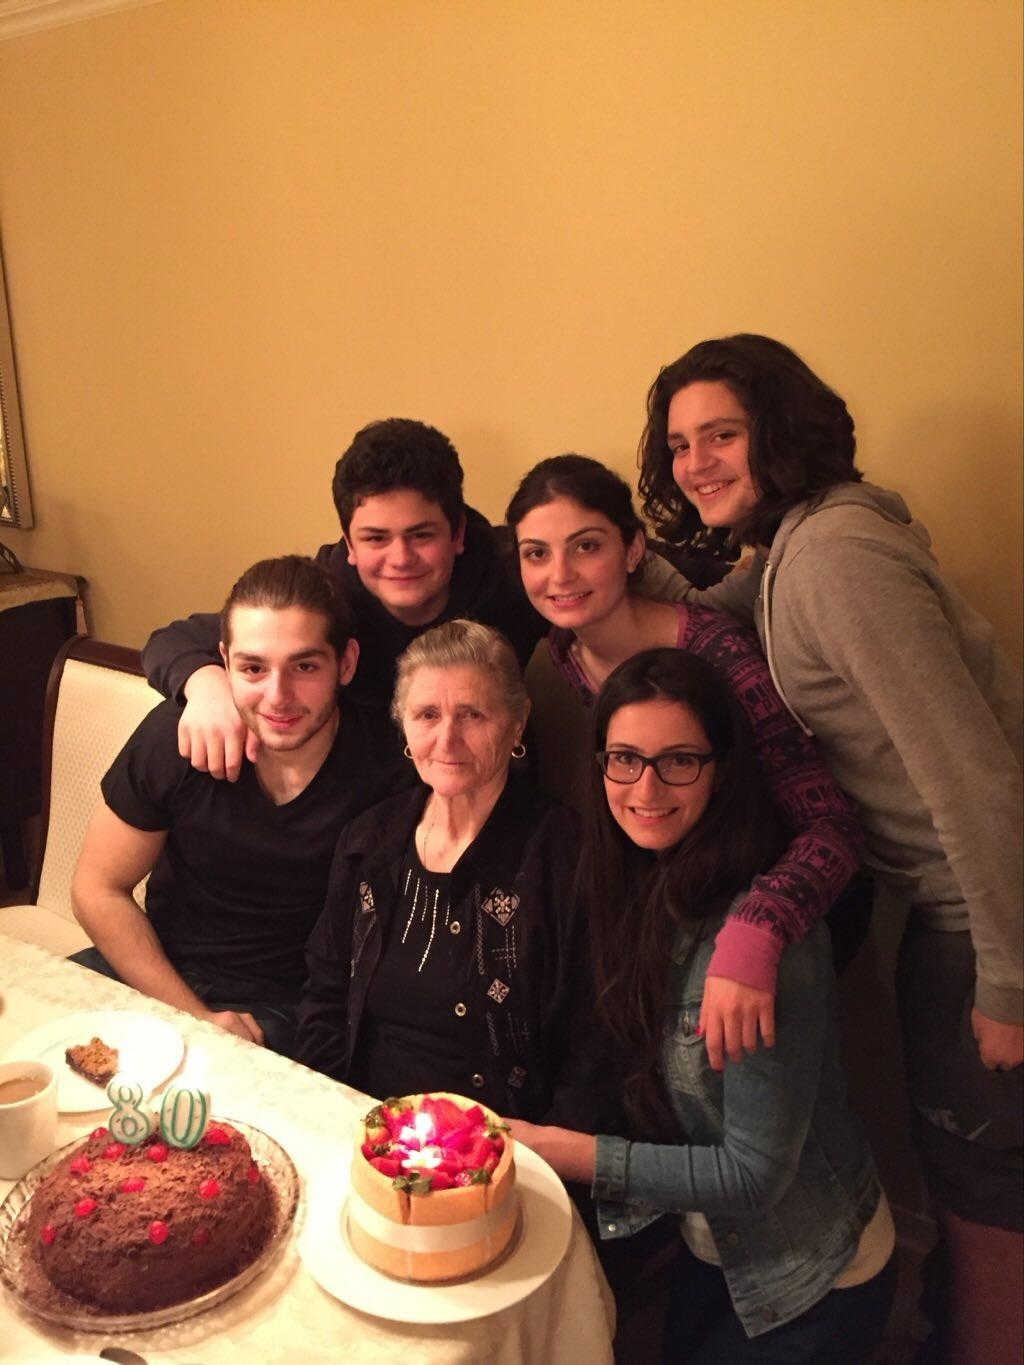
\includegraphics[width=60mm]{monanteras/images/Chocolate cake 2.jpg}
  \caption{Celebrating Grandma's 80^{th} birthday}
  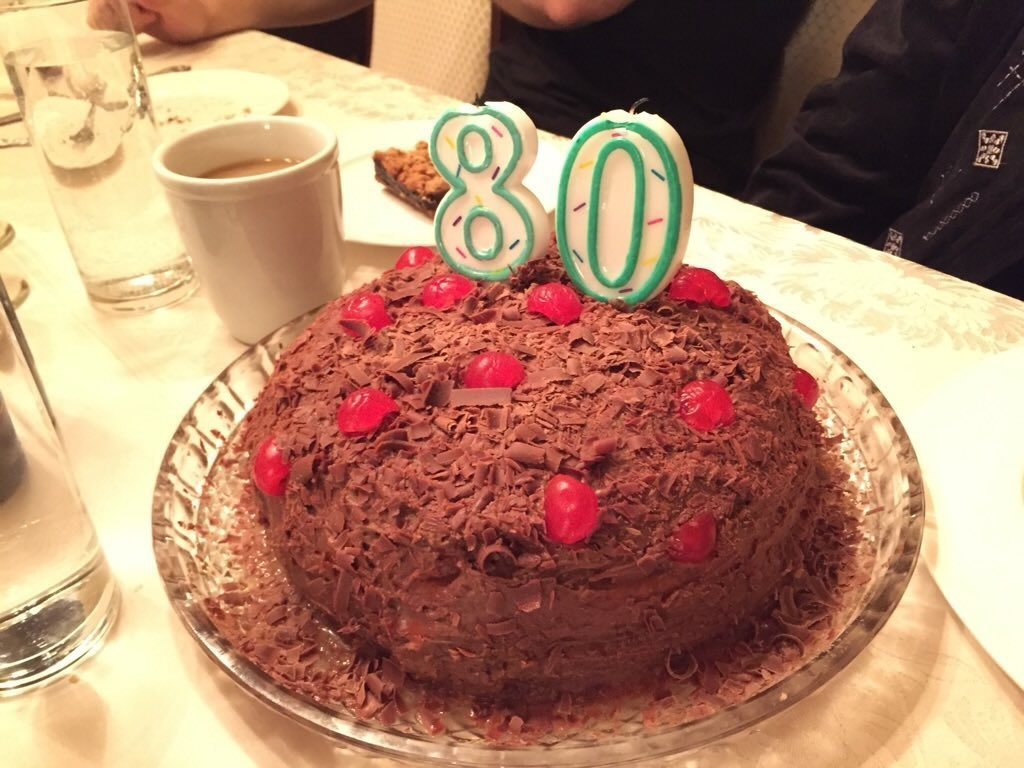
\includegraphics[width=60mm]{monanteras/images/Chocolate cake.jpg}
  \caption{The Chocolate Cake}
  \label{fig:fig}
\end{figure}

\newthought{Grandma Ελένη} 

\begin{enumerate}
    \item 
\end{enumerate}